\subsection{Sorting randomly generated objects}
\label{ssec:random_object_argsort}
\def\subtask#1{\noindent{\it\bfseries #1.}}


A natural type of relation on which to test our Abstractor models is \textit{ordering}. Suppose we have a set of $N$
objects $\mathcal{X} = \{ x_1 , ..., x_N \}$ with a strict ordering relation $x_1 \prec x_2 \prec \cdots \prec x_N$. The task is as follows: given a set of randomly permuted objects in $\mathcal{X}$, return the sorted sequence of objects according to the underlying ordering, by sorting their indices in the sequence---\texttt{argsort}.

The \texttt{argsort} task is a fully relational sequence-to-sequence task since it only requires relational
information (the ordinal values of the objects) to solve. We use this task to compare our proposed Abstractor models
to a standard Transformer.
Transformers are large and powerful sequence models. Given enough data, they can solve almost any task. We are interested in comparing the sample efficiency of our Abstractor models to Transformers, investigating how the Abstractor's
% natural capabilities of
inductive biases for modeling abstract relations allows it
%solve relational tasks more effectively and with fewer training samples than a Transformer.
% JDC: TRIED TO UNPACK AND BE MORE PRECISE ABOUT THE CLAIMS, WHICH I TOOK TO BE THE FOLLOWING.  HOWEVER, THE CLAIM
% ABOUT EFFECTIVENESS GIVES ME A BIT OF PAUSE, AS IT COULD BE CONSTRUED TO BE MORE ABOUT ASYMPTOTIC PERFORMANCE
% RATHER THAN PERFORMANCE AT *A GIVEN LEVEL OF TRAINING* (WHICH IS WHAT I BELIEVE WE CONSIDER IN THE SECTION ON
% GENERALIZATION) COULD BE CONSTRUED SIMPLY ANOTHER EXPRESSION OF DATA EFFICIENCY).  HOWEVER, ANOTHER WAY TO CONSTRUE
% EFFECTIVENESS MIGHT BE IN TERMS OF *REPRESENTATIONAL* EFFICIENCY (E.G., NUMBER OF PARAMETERS NEEDED?). THE LATTER
% IS SOMETHING WE MIGHT WANT TO ANALYSZE AND DISCUSS, IN THE CONTEXT OF BEING ABLE TO MAKE EMPIRICAL CLAIMS ABOUT
% SYMBOLIC BASIS OF PROCESSING.
learn relational tasks more effienctly (i.e., with fewer training samples) and more effectively (i.e., yielding
better generalization performance) than a Transformer

\subtask{Random object sorting task} We generate $N=64$ random objects as 8-dimensional Gaussian vectors, $\mathcal{X} = \{ x_1 , ..., x_{64} \}, \ x_i \overset{\mathrm{iid}}{\sim} \mathcal{N}(0, I) \in \reals^8$. We associate to them the ordering $x_1 \prec x_2 \prec \cdots \prec x_{64}$. The input sequences in the training data are randomly permuted sequences of $10$ objects in $\mathcal{X}$. The target sequences are the indices of the object sequences in sorted order (i.e., the `argsort'). The training data are sampled uniformly from $\{ X \in 2^\mathcal{X} \ \vert \ |X| = 10\}$. We also generate a validation dataset (used during training) and a testing dataset (used during evaluation).

\subtask{Model} We compare analogous configurations of a standard Transformer and a relational Abstractor. The sequence-to-sequence relational Abstractor is of the form $\texttt{Encoder} \to \texttt{Abstractor} \to \texttt{Decoder}$. The Encoder-to-Abstractor interface uses relational cross-attention and the Abstractor-to-Decoder interface uses standard cross-attention. The Abstractor and Transformer share the same hyperparameters: 2 layers (for each of the encoder, abstractor, and decoder), 2 attention heads, and a `model dimension' of 64.

\subtask{Evaluation of sample efficiency} We evaluate learning curves on this task for each model for training set
sizes ranging from $
100$ sequences to $3,000$ sequences in increments of $100$. For each training set size we run 10 trials each. Each trial consists of training a model on a dataset of the corresponding size for 200 epochs. Throughout training, performance metrics are tracked on both the training and validation datasets. The model from the best-performing epoch for that trial according to the validation dataset is restored and evaluated on the testing dataset. For each trial, we evaluate $\text{sequence sorting accuracy} = \frac{\text{\# of sequence sorted correctly}}{\text{Total \# of test set sequences}}$.

\subtask{Evaluation of task-generalization ability}
%One promise of the Abstractor framework is its ability to generalize
One reason the Abstractor may learn more efficiently is its ability to learn more abstract representations of relations, which generalize more effectively
 to new relational tasks. In particular, the relational bottleneck enables learning purely relational computations which are, in some sense, independent from the particular representations of the objects and hence would be applicable to new domains in which similar relational structures hold.
% JDC: IT WOULD BE GOOD TO TEST THIS DIRECTLY, BY EXAMINING THE PATTERNS OF ACTIVITY
% ASSOCIATED WITH THE ABSTRACTOR'S REPRESENTATIONS FOR A GIVEN STIMULUS / SET OF STIMULI IN A GIVEN ROLE;  WE CAN MAKE
% THE STRONG PREDICTION THAT THERE SHOULD BE LOWER VARIANCE IN SUCH REPRESENTATIONS OVER INSTANCES OF COMPUTING A
% GIVEN RELATION THAN FOR THE TRANSFORMER, WHICH IS AN IMPORTANT HALLMARK OF SYMBOLIC COMPUTATION (AND I WISH WE
% COULD APPLY TO LLMs!!)
We test the Abstractor's ability to achieve such generalization on the object sorting task in the following way. We
generate a second object-sorting dataset by independently sampling a new set of random objects, $\mathcal{X} = \{ \tilde{x}_1 , ..., \tilde{x}_{64} \}, \ \tilde{x}_i \overset{\mathrm{iid}}{\sim} \mathcal{N}(0, I) \in \reals^8$. We train a relational Abstractor model on 10,000 sequences of the second sorting task. We additionally evaluate learning curves for a relational Abstractor in which the weights of the abstractor module are initialized and fixed to be those of the abstractor module from the second sorting task (while keeping the encoder and decoder trainable).
% JDC: I GATHER THE LATTER IS A (BETTER CONTROLLED) PROXY FOR A "BASELINE TRANSFORMER" MODEL.  MIGHT BE GOOD TO MAKE
% THAT EXPLICIT.  MIGHT ALSO WANT TO ADD CONTINUED TRAINING ("FINE TUNING") OF THE BASELINE TRANSFORMER, JUST FOR
% COMPLETENESS.
We evaluate whether this results in improved sample efficiency.

\begin{figure}[t!]
	\centering
	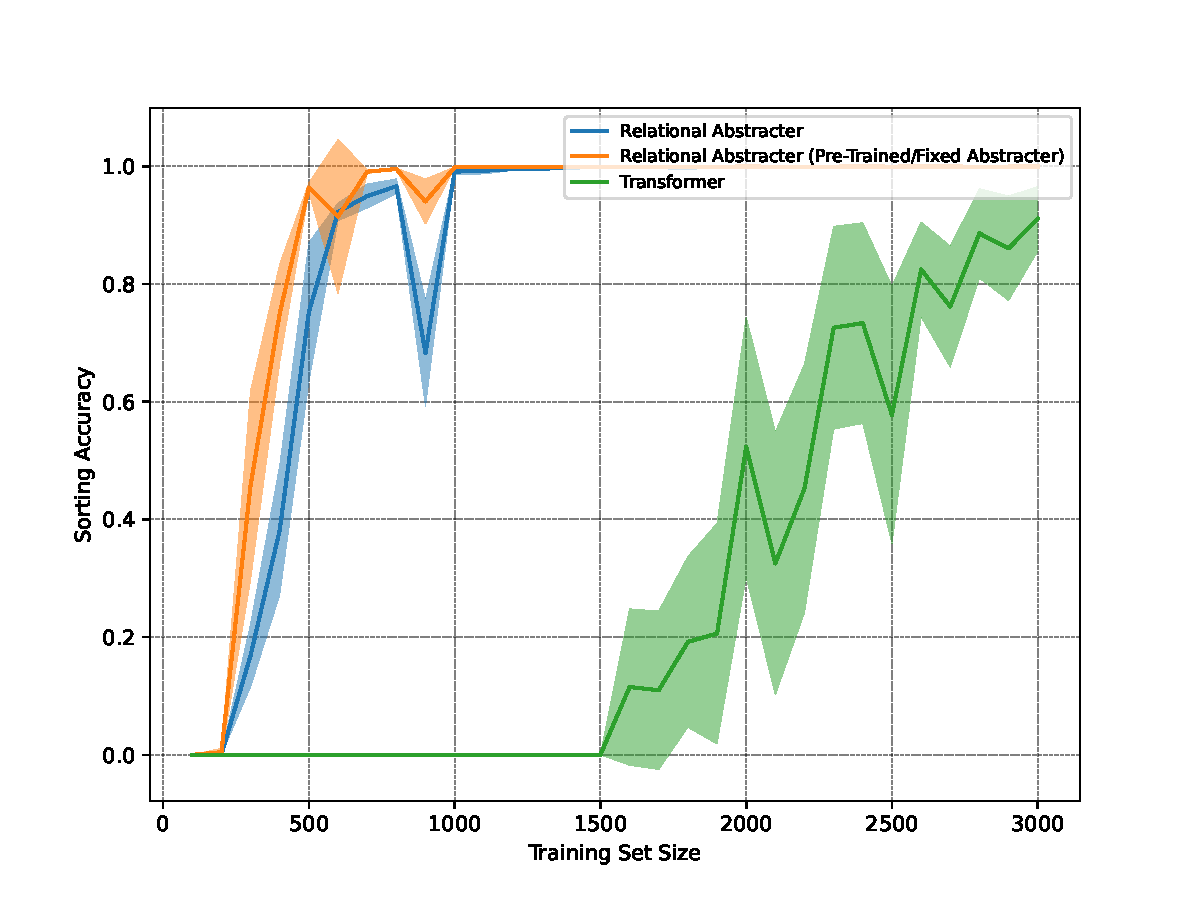
\includegraphics[width=.8\textwidth]{figures/random_object_argsort_learning_curves.pdf}
	\caption{Learning curves of three model configurations: a Transformer, a relational Abstractor, and a relational Abstractor in which the abstractor module is pre-trained on an independent sorting task. The lines indicate the mean sorting accuracy over 10 trials for that training set size, and the shaded region indicates two times the standard error of mean. Sorting accuracy is evaluated on an independent testing set at the end of a trial.}
	\label{fig:random_object_argsort_learning_curves}
\end{figure}


The learning curves for each model configuration are shown in \Cref{fig:random_object_argsort_learning_curves}. We observe that the relational Abstractors have significantly improved sample efficiency for this task over a standard Transformer. In fact, with training set sizes between 1,000-1,500 sequences, the Abstractors can perfectly perform the task while the Transformer fails to sort any sequences in the testing dataset fully correctly. We also observe reduced trial-to-trial variability in model performance in the Abstractors.
% JDC: THE LATTER MAY RELATE CLOSELY TO THE POINT MADE ABOVE (ABOUT THE CONSISTENCY OF THE REPRESENTATIONS AS
% EVIDENCE OF SYMBOLIC COMPUTING)
The relational Abstractor with a pre-trained abstractor module displays a small improvement in sample efficiency and a further reduction in the sample-to-sample variability of model performance.

